
\begin{frame}
  \maketitle
\end{frame}

\section{本編}
\begin{frame}{背景と目的}
  \begin{itemize}
  \item マルチホップ通信$\cdots$通信のタイミングや通信先の予測は困難
  \item 単純に平均頂点間距離が小さいトポロジが有効
    \cite{Koibuchi2012, Singla2011}
  \item \alert{一般化ムーアグラフ}
    \begin{itemize}
    \item 平均頂点間距離が理論的な下界に等しい正則グラフ
      \cite{cerf1973computer, Cerf1974}
    \end{itemize}
  \item 発見する方法はいくつかある
    \cite{Fujita2015, Yamamoto2016}
  \item グラフの性質を利用した探索法は知られていない
  \end{itemize}
  \begin{columns}[T]
    \begin{column}{.4\textwidth}
      \begin{block}{}
        全探索をベースにして比較的に効率よく探索する方法を提案・検証
      \end{block}
    \end{column}
    \begin{column}{.4\textwidth}
      \begin{figure}
        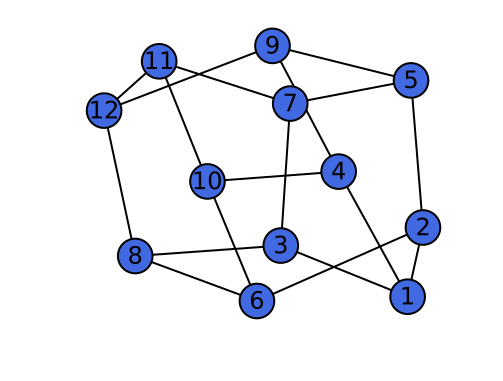
\includegraphics[width=.8\linewidth]{gmg-example-bignode}
        \caption{一般化ムーアグラフの例}
      \end{figure}
    \end{column}
  \end{columns}
\end{frame}

\begin{frame}{方法}
  \begin{enumerate}
  \item 与えられた頂点数と次数の初期グラフを構築しておく
  \item 図\ref{fig:feasible-edges-example}の赤の辺から
    逐次辺取り出して追加できるか求める
    \begin{itemize}
    \item 図\ref{fig:feasible-edges-example2}では
      最小の閉路長が$5$以上のとき追加可能
    \item $a$,$b$,$c$のうち$c$のみが追加可能
    \end{itemize}
  \end{enumerate}
  \begin{itemize}
  \item 初期グラフを変えることで探索を高効率化
  \end{itemize}
  \begin{figure}
    \centering
    \begin{minipage}{.4\columnwidth}
      \def\svgwidth{\textwidth}
      \input{feasible-edges-example-color.pdf_tex}
      \captionof{figure}{初期グラフの例と辺の候補}
      \label{fig:feasible-edges-example}
    \end{minipage}
    \hspace{1em}
    \begin{minipage}{.4\columnwidth}
      \def\svgwidth{\textwidth}
      \input{feasible-edges-example2-color.pdf_tex}
      \captionof{figure}{探索途中のグラフ}
      \label{fig:feasible-edges-example2}
    \end{minipage}
  \end{figure}
\end{frame}

\begin{frame}{現在までの成果}
  \begin{columns}
    \begin{column}{.6\textwidth}
      \centering
      \begin{itemize}
      \item 全域木からの探索が効率的
      \end{itemize}
      \includegraphics[height=.5\textheight]{mid-cmp-algo-time}
      \captionof{figure}{次数=3の結果 \\ {\scriptsize
          探索開始から最初の一般化ムーアグラフを発見するまでの時間を表す.
          探索を10回行い,実行時間の平均を計算した.
      }}
      \label{fig:result}
    \end{column}
    \begin{column}{.4\textwidth}
      \centering
      \begin{figure}
        \centering
        \def\svgwidth{\textwidth}
        \resizebox{!}{.3\textheight}{
          \input{initial-tree-cycle-example.pdf_tex}
        }
        \caption{閉路を含む初期グラフ}
        \label{fig:initial-graph-cycle}
      \end{figure}
      \vspace{-2em}
      \begin{figure}
        \def\svgwidth{\textwidth}
        \resizebox{!}{.3\textheight}{
          \input{initial-spanning-tree-12-example.pdf_tex}
        }
        \captionof{figure}{全域木}
        \label{fig:initial-graph-stree}
      \end{figure}
    \end{column}
  \end{columns}
\end{frame}

\begin{frame}{今後の課題}
  \begin{itemize}
  \item より効率的な探索方法の提案
  \item 予想の証明
    \begin{itemize}
    \item 一般化ムーアグラフの部分グラフに,図\ref{fig:initial-graph-cycle}
      に示したようなグラフが存在する.
    \item 一般化ムーアグラフの全域木に,図\ref{fig:initial-graph-stree}
      に示したような木が存在する.
    \end{itemize}
  \item 同型グラフ判定を用いた列挙
  \item 一般化ムーアグラフが存在しない場合の考察
  \end{itemize}
\end{frame}

\appendix
\begin{frame}<handout:0>{一般化ムーアグラフの条件}
  \begin{thm}
    正則グラフが一般化ムーアグラフであることの必要十分条件は,
    \begin{itemize}
    \item 長さ$2Q$以下の閉路が存在しない
    \item 直径が$Q+1$である($Q+1$層に頂点が存在しない場合は$Q$)
    \end{itemize}
    を同時に満たすことである.
  \end{thm}
  \begin{figure}
    \centering
    \def\svgwith{.4\textwidth}
    \resizebox{.4\textwidth}{!}{
      \input{initial-tree-example.pdf_tex}
    }
    \caption{高さ$Q=2$の木}
  \end{figure}
\end{frame}

\begin{frame}<handout:0>{発見した一般化ムーアグラフの数の比較}
  \begin{columns}
    \begin{minipage}[t]{.5\textwidth}
      \centering
      \includegraphics[height=.65\textwidth]{mid-cmp-algo-full-graph}
      \captionof{figure}{発見したグラフの数 \\ {\scriptsize
          なお,同型なグラフは重複して数えている.
      }}
      \label{fig:full-graph}
    \end{minipage}
    \hspace{1ex}
    \begin{minipage}[t]{.5\textwidth}
      \centering
      \includegraphics[height=.65\textwidth]{mid-cmp-algo-full-time}
      \captionof{figure}{グラフ1個の発見に要した時間 \\ {\scriptsize
          すべてのグラフの発見に要した時間を図\ref{fig:full-graph}の値で
          割った値である.
      }}
      \label{fig:full-time}
    \end{minipage}
  \end{columns}
\end{frame}

\begin{frame}[allowframebreaks]{参考文献}
  \bibliography{../resource/MyCollection}
\end{frame}

